% 1. fact check claim that other brain parcellation studies use
%    Pearson's correlation (not absolute value) as edge weights
%#######################################################################

Functional parcellation of the human brain can be defined as the problem
of partitioning the voxels into $k$ disjoint connected components with
the goal that the voxels within each component are, in a rough sense,
\"similar\" to each other and voxels in different components are less
\"similar\". Such similarity has been defined in a multitude of ways in
the literature [see lit review section ...]. For this project thus far I
have taken similarity between voxels to mean statistical dependence.

To measure dependence, statisticians have traditionally used the Pearson
correlation coefficient, in addition to the rank-based Kendall tau and
Spearman rho. These statistics work well when the underlying
relationship between the two random variables is linear, in the case of
Pearson, or can be linear after a monotonic transformation, in the case
of Kendall and Spearman. Due to their restrictions, these correlation
coefficients will fail to capture many kinds of dependency
relationships. The figure below illustrates several instances of pairs
of random variables whose depencency structure is not detected by the
three correlation coefficients.

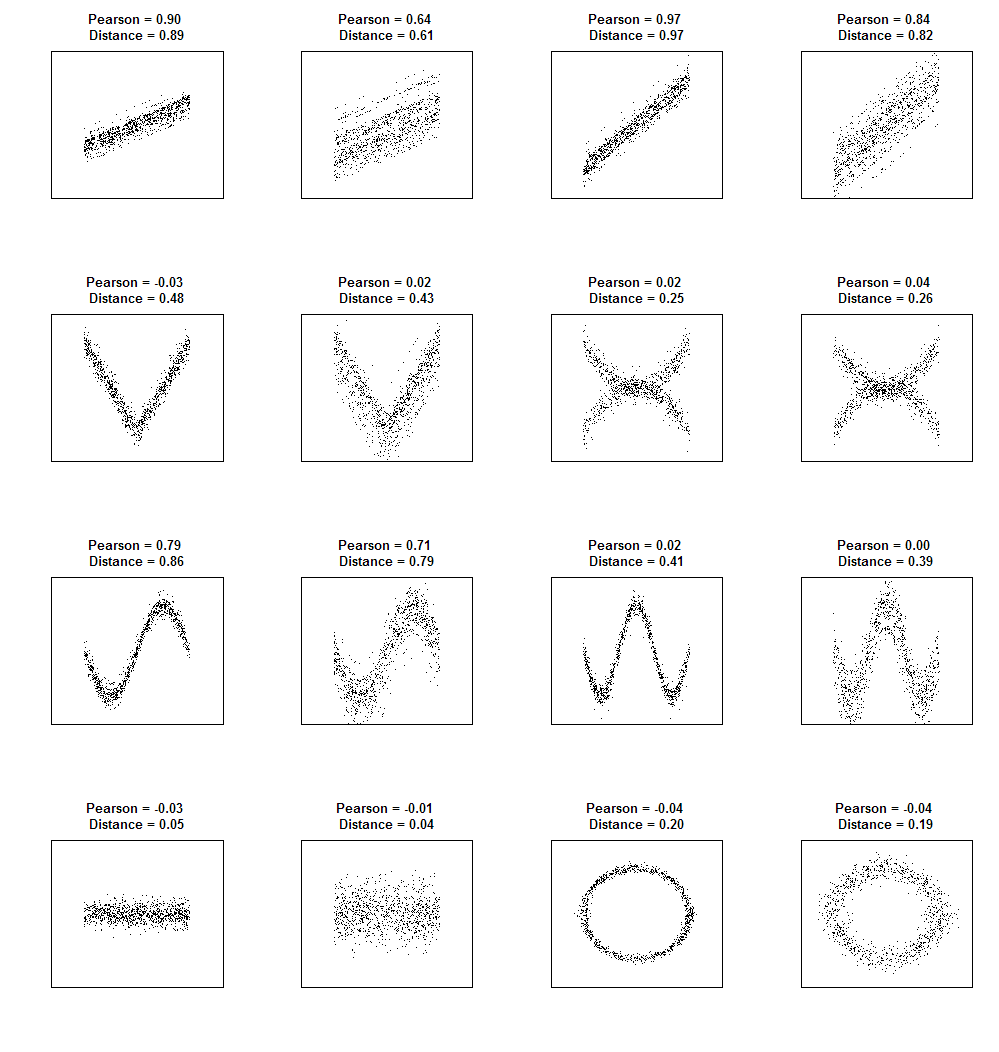
\includegraphics[scale = 0.8]{1_nonlinear_depend.png}

Non-linear dependency relationships also exist in the ABIDE 50002 fMRI
data. The scatterplots below show time samples of spatially adjacent
voxels. These instances were found by searching for the maximum
difference in rank of energy distance correlation and the coefficient
of determination, or Pearson squared.

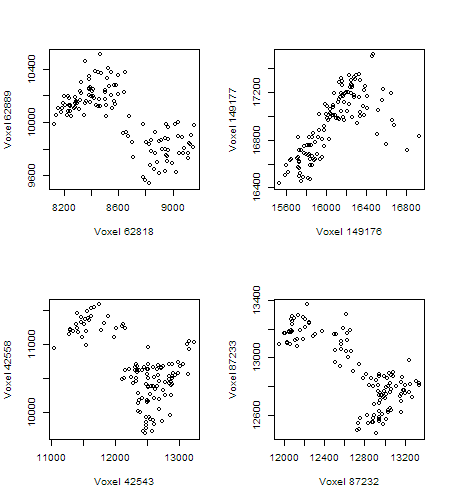
\includegraphics[scale = 0.7]{1_nonlinear_ABIDE_50002.png}

Many studies on functional parcellation (Craddock 2012; Bellec 2006;
Heller 2006) use Pearson's coefficient as the similarity measure between
nearby voxels. Apart from underestimating the important of non-linear
relationships, this method also distinguishes positive, upward-sloping
correlation from negative. As a result in many of the edges between
different parcels, the corresponding voxels would be strongly dependent
with negative correlation.

In this investigation, all parcellation and validation procedures were
conducted on the ABIDE 50002 fMRI data set. This data set contains
233305 voxels and 124 time samples. Spatial information is encoded as a
graph; each voxel is represented by a vertex, and each vertex has up to
6 edges connecting the voxel to its cubically adjacent neighbors. The
weights on the edges are sample energy distance correlations between the
two connected voxels (Szekely 2013).
